\section{Datapath}

\begin{figure}[H]
      \centering
      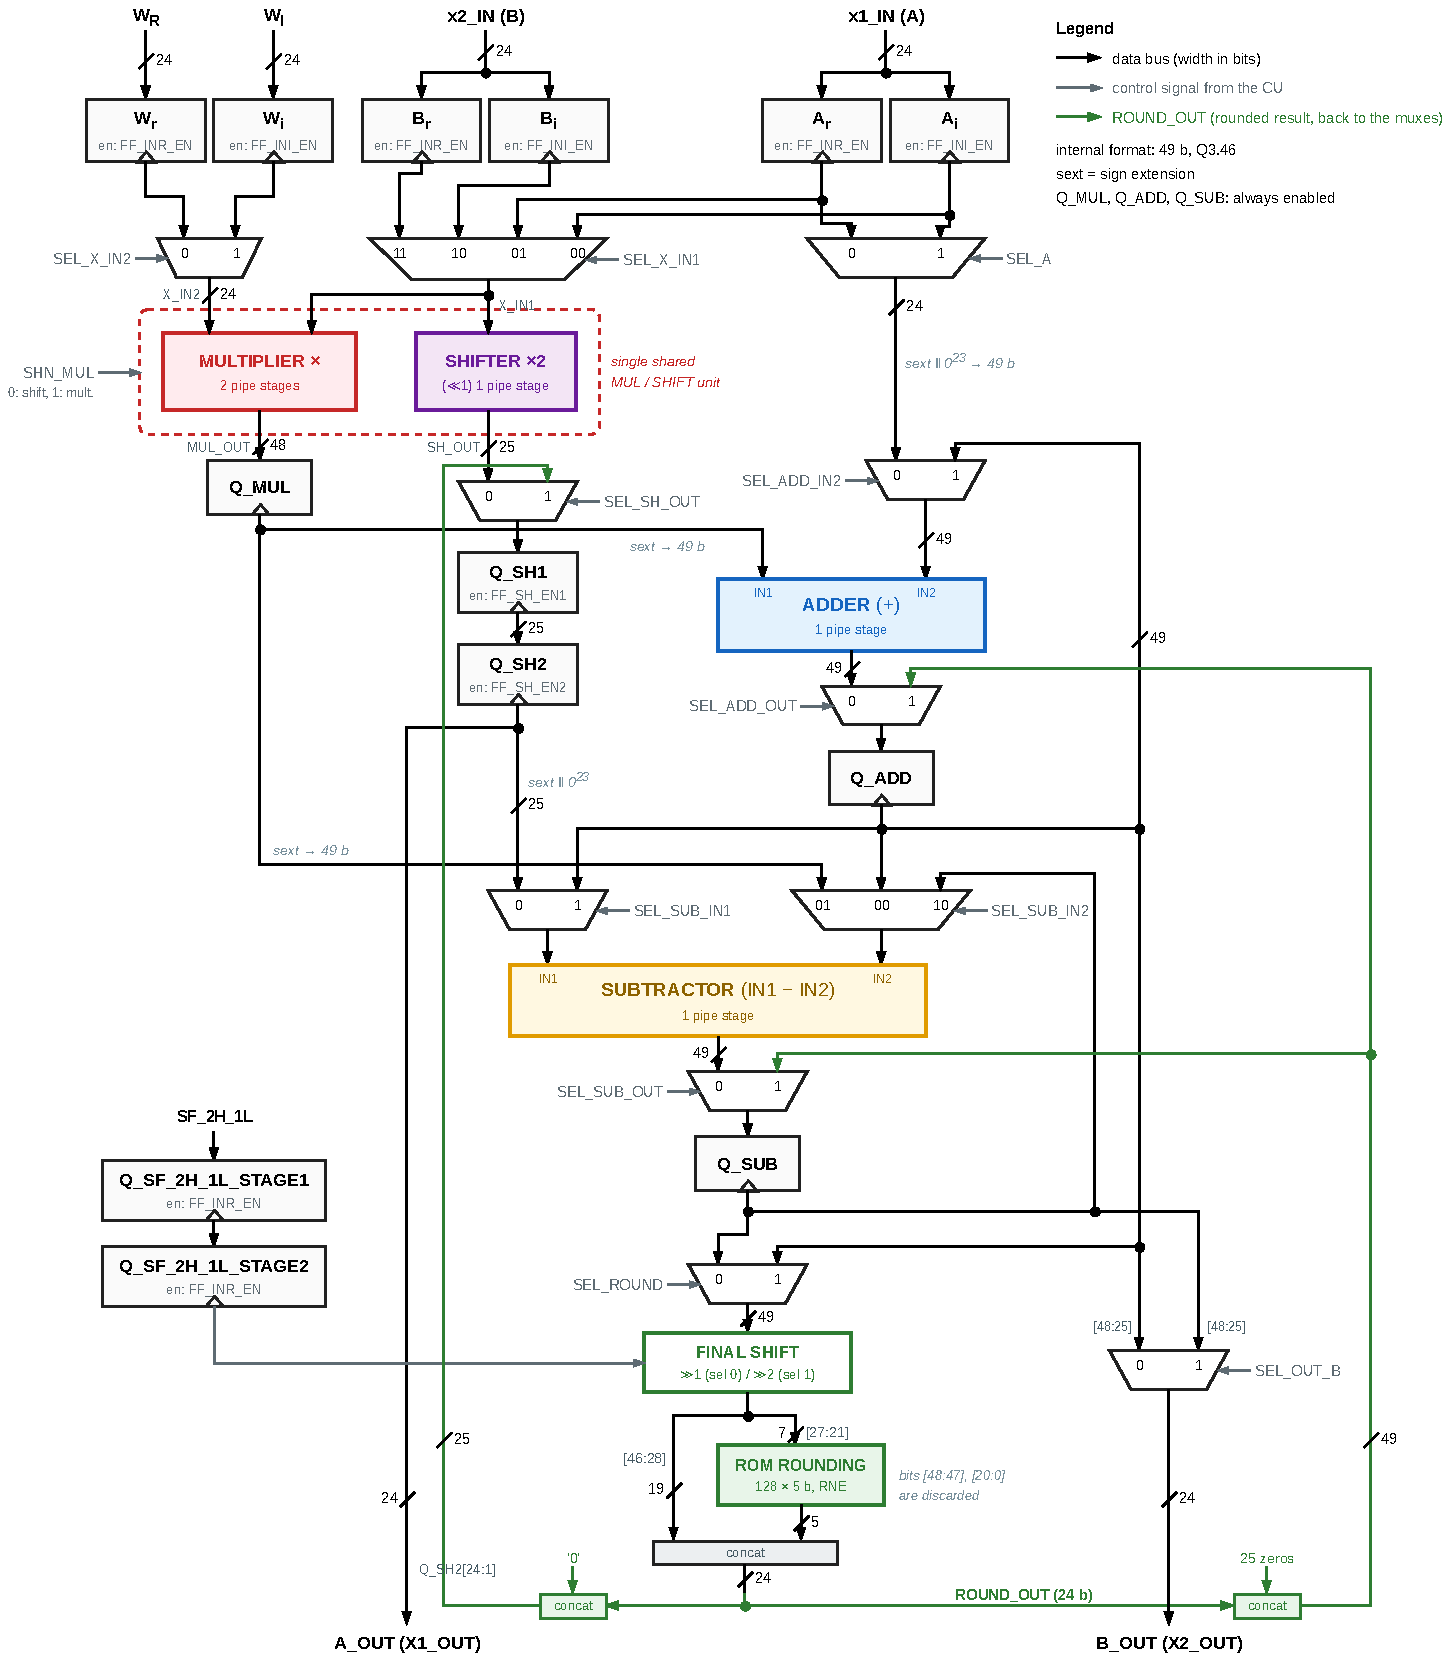
\includegraphics[width=1\textwidth]{fig03_datapath}
      \caption{Datapath dell'unità butterfly}
\end{figure} 

\noindent L'interfaccia in ingresso si occupa di acquisire i dati complessi di input A, B ed i coefficienti di rotazione W. Come richiesto dalle specifiche, per parallelizzare il caricamento dei valori, i bus di ingresso di A e B sono separati. Si introducono due registri per ogni parametro A, B, W, uno per la parte reale ed uno per la parte immaginaria. Essi sono abilitati da specifici segnali di controllo e servono a campionare i dati in ingresso, mantenendoli stabili durante l'elaborazione della butterfly. Per il parametro W, la parte reale ed immaginaria entrano su due porte differenti. Essendo disponibile, invece, un singolo canale di ingresso per A ed uno per B, si suppone che, per ciascun dato, si invii inizialmente la parte reale e, successivamente, quella immaginaria. Il segnale in arrivo dall'unità di controllo $FF\_INR\_EN$ attiva i registri relativi alle componenti reali, mentre $FF\_INI\_EN$ quelli delle componenti immaginarie.

\noindent Per le componenti A, vi è un multiplexer, che, in base al valore del segnale $SEL\_A$, invia verso un secondo multiplexer la sua parte reale od immaginaria.

\noindent Le specifiche del progetto impongono l'uso di un solo moltiplicatore, un sommatore ed un sottrattore.

\noindent  Il primo può operare in due modalità distinte (prodotto canonico o shift aritmetico verso sinistra, al fine di compiere un raddoppio del dato al suo ingresso), selezionate dal segnale SHN\_MUL (ovvero SHN\_MUL: 0 = shift, 1 = moltiplicazione). L'uscita del moltiplicatore è salvata nel registro che ha come uscita $Q\_MUL$, procedimento necessario per sincronizzare il risultato del blocco con il resto del sistema; il risultato della moltiplicazione arriva dopo due colpi di clock a causa della sua pipeline interna.
Dal momento che si lavora in fixed point, il prodotto di due numeri a 24 bit ne produce 48. Il datapath interno mantiene la precisione estesa (grazie a un parallelismo di 49 bit, come descritto nella sottosezione seguente), senza alcun arrotondamento fino allo stadio finale. Inoltre, in ingresso, è posto un multiplexer a quattro ingressi, con segnale di controllo $SEL\_X\_IN1$, che seleziona su quale componente di A o B operare, ed un multiplexer a due vie, con selettore $SEL\_X\_IN2$, che sceglie tra la parte reale od immaginaria di W, le quali risultano utili unicamente all'esecuzione del prodotto.
    
\noindent  Per quanto riguarda il sommatore, come ingresso presenta sicuramente il risultato del moltiplicatore $Q\_MUL$, che prende il nome di $ADD\_IN1$. In aggiunta, il controllo $SEL\_ADD\_IN2$ coordina se sommargli i dati provenienti dai registri di ingresso di A o il risultato interno parziale del sommatore stesso. L'uscita del sommatore, se $SEL\_ADD\_OUT$ vale 0, viene salvata nel registro dedicato, la cui uscita è denominata $Q\_ADD$.
    
\noindent  Come richiesto da specifiche, il sottrattore è un blocco diverso dal sommatore. L'uscita viene memorizzata nel registro con output $Q\_SUB$ se si verifica che $SEL\_SUB\_OUT = 0$. Analogamente al blocco ADD, in ingresso presenta due multiplexer, uno a due ingressi ed uno a quattro, i cui rispettivi selettori $SEL\_SUB\_IN1$ e $SEL\_SUB\_IN2$ selezionano gli operandi appropriati. Il primo multiplexer può ricevere $Q\_ADD$ oppure una componente shiftata verso sinistra; il secondo, invece, ha come ingressi $Q\_ADD$, $Q\_MUL$ o il risultato parziale della sottrazione.


\noindent Infine, si ha un ulteriore multiplexer di selezione (con segnale di controllo $SEL\_ROUND$) che instrada i risultati intermedi provenienti dal Sommatore e dal Sottrattore, al fine di ottenere i risultati da fornire in uscita $A'_{r}$, $A'_{i}$, $B'_{r}$, $B'_{i}$, successivamente a uno shift finale e all'arrotondamento. Avendo un'unica unità di arrotondamento, i dati da approssimare devono essere serializzati, come già visto durante l'analisi del Data Flow Diagram.

\noindent Successivamente a tale multiplexer, è inserito un blocco, denominato final shifter, che implementa l'Unconditional Block Floating Point Scaling richiesto, con l'obiettivo di riportare il numero considerato nell'intervallo (-1;+1). Dall'esterno viene fornito un SF\_2H\_1L: se esso vale zero, il blocco scala di una posizione, se è uno, si shifta a destra di due. Poiché, come si vedrà nella sezione seguente, si riceve tale segnale insieme alle parti reali dei dati in ingresso, è necessaria una catena di registri in serie, pilotati dal segnale $FF\_INR\_EN$, al fine di garantire un corretto funzionamento del Right shift.

\noindent Infine, il ROM Rounding (in verde) svolge l'approssimazione Round To Nearest Even. Per facilitare la visualizzazione di dove i valori arrotondati verranno salvati, questi ultimi si sono indicati in verde in corrispondenza dei registri in cui verranno salvati.

\noindent In particolare, dall'analisi del DFD e del datapath, si osserva che è possibile salvare le componenti delle uscite $A'_r$ e $A'_i$ all'interno dei 2 registri a cascata presenti al di sotto dello shifter aritmetico, che salva ed accumula le componenti di A'. Prima viene ricevuta la parte reale, che viene salvata nel primo registro. Al ciclo successivo, questa transisce nel FF adiacente, mentre il primo campiona $A'_{i}$. Invece, le uscite $B'_r$ e $B'_i$ vengono salvate, rispettivamente, nei registri sottostanti al sommatore e al sottrattore.

\noindent Infine, $A\_OUT$ e $B\_OUT$ sono i punti in cui vengono fornite le uscite. In corrispondenza della seconda, è anche presente un multiplexer con selettore $SEL\_OUT\_B$, che smista i dati ricevuti dai due registri in cui sono salvabili le uscite $B'_r$ e $B'_i$.

\noindent Tutto il sistema è sincronizzato da un clock comune (clk).
Una delle richieste del progetto chiedeva inoltre di limitare il tempo di vita delle variabili ed il numero di connessioni tra gli elementi a patto di non penalizzare le prestazioni, e questo ha portato all’ottimizzazione dei registri visti in precedenza e alla progettazione di questi snodi per il campionamento delle uscite, allungando le interconnessioni presenti nell'architettura. L’idea dietro a questa scelta è che, poiché gli elementi da connettere sono molto ravvicinati, si potrebbe ottenere un miglior risultato diminuendo al minimo il numero dei registri (i quali hanno un parallelismo non indifferente) e le loro connessioni e di conseguenza l’area. In alternativa,  si potrebbero salvare le 4 uscite su degli appositi registri posizionati a valle dell'arrotondamento, per non dover spostare tali dati,  con l'ovvio svantaggio di un numero di registri maggiore nell'architettura.

\subsection{Parallelismo interno}

Nello schema sono state inserite le indicazioni sul numero di bit dei segnali rilevanti. Come da specifica, i dati in ingresso, come quelli di uscita, sono su 24 bit.
Il registro all’uscita della moltiplicazione è da 48 bit (di cui il MSB è un bit per evitare overflow, per gestire anche il caso limite $-1 \cdot -1$), mentre in uscita allo shift aritmetico sono due registri in cascata che presentano 25 bit. Al fine di evitare overflow, è necessario aumentare il parallelismo interno. Per tale ragione, poiché a livello teorico non ci si aspetta più di 2 overflow, è sufficiente utilizzare un parallelismo di 49 bit. Tutti i dati prima di esser usati dal sommatore e dal sottrattore sono portati, se necessario, a tale parallelismo, aggiungendo un numero appropriato di 0 a destra (23, per i risultati dello shifter aritmetico e per le componenti di A da fornire al sommatore) e estendendo il segno a sinistra; in questo modo, si garantisce di lavorare su dati intermedi nella medesima codifica fixed point Q3.46. Questo meccanismo serve per mantenere la massima precisione senza troncamento durante i calcoli intermedi, come richiesto, prima di arrivare al blocco di FINAL SHIFT e ROM Rounding.

\subsection{Blocco di FINAL SHIFT e ROM ROUNDING}
Al termine delle operazioni, i dati ottenuti con un parallelismo di 49 bit vengono shiftati verso destra di una o due posizioni, in base al segnale SF\_2H\_1L, applicando l’estensione del segno per i bit aggiunti da sinistra. Per questo motivo, al momento dell’arrotondamento, è conveniente scartarli e prelevare i dati a partire dal bit 46-esimo, al fine di ristabilire il range dinamico corretto. 

\noindent Per tale ragione, al fine di ottenere dei risultati codificati su 24 bit, si sceglie di considerare la finestra di bit “46 downto 21” del segnale in uscita al Right Shifter (denominato nel file VHDL del datapath come SHIFT\_mux\_OUT). Questa finestra ha un'ampiezza maggiore di 24 bit, questo poiché non si effettua il troncamento netto dei bit meno significativi ma si ricorre ad un arrotondamento dei dati mediante la tecnica del Round to Nearest Even, implementata tramite un ROM Rounding.
In particolare, all'interno del blocco di Rounding, entrano unicamente i bit “27 downto 21”, poiché si è scelto di sviluppare un approssimatore attraverso una ROM che ha 7 bit in indirizzo (“27 downto 21”) e parole da 5 bit. Perciò, l'arrotondamento implementato scarta i due bit, mentre sui primi 5 viene effettuato un incremento di un'unità, quando richiesto. In particolare, l'incremento è sempre dovuto se i due bit meno significativi sono entrambi alti; invece, se sono "10", si ha un incremento unicamente se il terzo bit meno significativo è alto (numero dispari).

\noindent I 5 bit in uscita dal blocco di Rounding si vanno a concatenare con i 19 bit più significativi originali (“46 downto 28”), componendo in tale modo il risultato su 24 bit, come richiesto dalle specifiche. In particolare, gli errori introdotti per i casi in cui i 5 bit significativi in ingresso  sono codificati in decimale con i numeri da 0 a 29 si compensano perfettamente. Ciò non risulta vero per il valore 30 (11110) e 31 (11111), che introducono rispettivamente un errore non bilanciato di -0.5 LSB e -1.5 LSB.

\noindent Si ottiene quindi un $$Errore\_{Totale} = (Sum_{0-29}) + Sum_{30} + Sum_{31} = 0\ LSB + (-0.50\ LSB) + (-1.50\ LSB) = -2.00\ LSB$$ e si ha di conseguenza un $$Bias\_Error = \frac{-2.00\ LSB}{128} \approx -0.0156\ LSB$$ 
Poiché il LSB dei risultati vale $2^{-23}$, in definitiva il bias error è pari a $-1.862645 \cdot 10^{-9}$. In assenza di rigide specifiche legate all'accuratezza dei risultati, si è supposto che tale errore fosse accettabile. Ovviamente, a seconda delle specifiche dell'applicazione di tale unità, si potrebbe valutare di modificare le dimensioni del ROM Rounding.

\begin{comment}
\noindent La ROM è programmata affinché implementi la logica per cui dato un dato dispari con il primo bit di scartato a ’1’, consegue l’incremento di un’unità dei bit “27 downto 23”,
I bit più significativi (“46 downto 28”) passano inalterati in uscita.
I 5 meno significativi (“27 downto 23”, che si suppone essere quelli che, con più probabilità, verrebbero modificati se ricevessero il ’+1’ dell’arrotondamento) insieme ai primi 2 bit scartati (“22 downto 21”, i quali permettono di decidere se arrotondare o no), invece, entrano nella ROM di arrotondamento. La ROM è programmata come una lookup table che implementa la logica per cui dato un dato dispari con il primo bit di scartato a ’1’, consegue l’incremento di un unità dei bit “27 downto 23”, al contrario cerco di tenere più a lungo i dati pari avendo in media 5 arrotondamenti sui valori sui pari e 3 sui dispari. Ovviamente se quest’ultima condizione non fosse rispettata i bit non verrebbero modificati.
Questi 5 bit vanno a sostituire i bit originali nel bus di uscita finale, per ricomporre il dato finale a 24 bit.
Otteniamo quindi un $$Errore_{Totale} = (Sum_{0-29}) + Sum_{30} + Sum_{31}= 0 + (-0.50) + (-1.50) = -2.00$$ e di conseguenza un $$Bias = \frac{-2.00}{128} = -0.0156\ LSB$$ e sapendo che 1 LSB $= 2^{-23}$ il bias vale $= 1.862645 \cdot 10^{-8}$.
\end{comment}
